\documentclass{standalone}
\usepackage{tikz}
\usetikzlibrary{shapes.geometric, arrows.meta, positioning, calc}
\usepackage{amsmath}
\usepackage{amsfonts}
\usepackage{noto} % Reliable font for PDFLaTeX, loaded last

% Define styles for blocks and arrows
\tikzstyle{block} = [rectangle, draw, fill=blue!20, 
    text width=6em, text centered, rounded corners, minimum height=4em]
\tikzstyle{input} = [coordinate]
\tikzstyle{output} = [coordinate]
\tikzstyle{noise} = [circle, draw, fill=red!20, inner sep=2pt]
\tikzstyle{arrow} = [thick, -Stealth, >=stealth]

\begin{document}

% Creating the block diagram
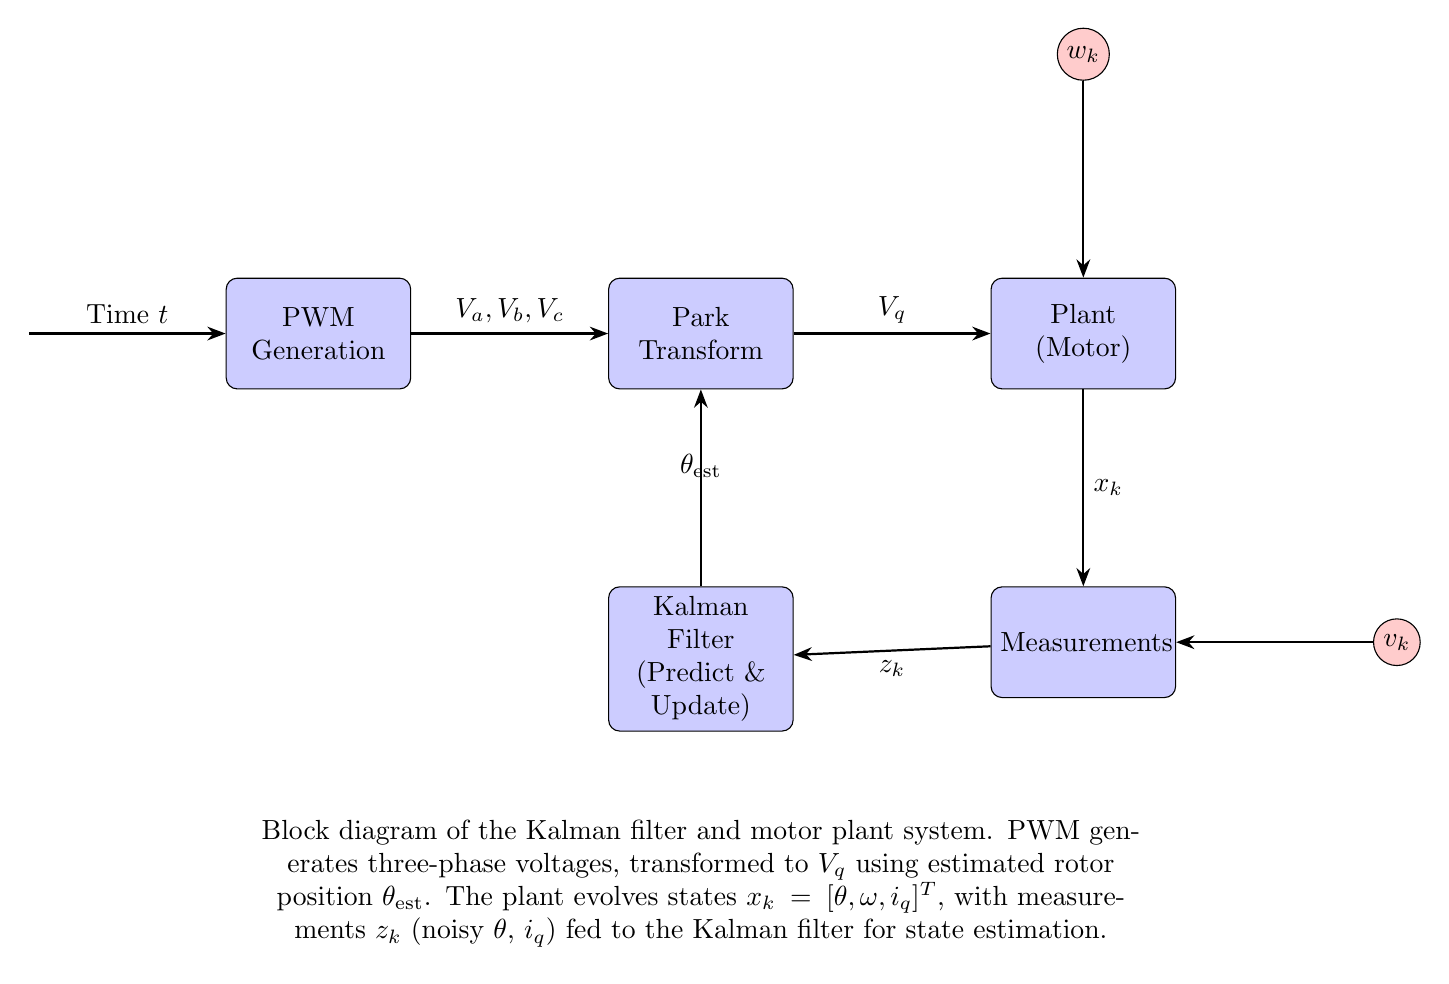
\begin{tikzpicture}[node distance=2.5cm, auto]
    % Define blocks
    \node [block] (pwm) {PWM Generation};
    \node [block, right=of pwm] (park) {Park Transform};
    \node [block, right=of park] (plant) {Plant (Motor)};
    \node [block, below=of plant] (meas) {Measurements};
    \node [block, below=of park] (kalman) {Kalman Filter\\(Predict \& Update)};
    
    % Noise nodes
    \node [noise, above=of plant] (w_noise) {$w_k$};
    \node [noise, right=of meas] (v_noise) {$v_k$};
    
    % Input and output coordinates
    \node [input, left=of pwm] (input) {};
    \node [output, right=of plant] (output) {};
    
    % Arrows for signal flow
    \draw [arrow] (input) -- node {Time $t$} (pwm);
    \draw [arrow] (pwm) -- node {$V_a, V_b, V_c$} (park);
    \draw [arrow] (park) -- node {$V_q$} (plant);
    \draw [arrow] (w_noise) -- (plant);
    \draw [arrow] (plant) -- node {$x_k$} (meas);
    \draw [arrow] (v_noise) -- (meas);
    \draw [arrow] (meas) -- node {$z_k$} (kalman);
    
    % Feedback loop for theta_est
    \draw [arrow] (kalman.north) -| node[pos=0.75, above] {$\theta_{\text{est}}$} 
        (park.south);
    
    % Caption below
    \node [below=1cm of kalman, align=center, text width=12cm] 
        {Block diagram of the Kalman filter and motor plant system. PWM generates three-phase voltages, transformed to $V_q$ using estimated rotor position $\theta_{\text{est}}$. The plant evolves states $x_k = [\theta, \omega, i_q]^T$, with measurements $z_k$ (noisy $\theta$, $i_q$) fed to the Kalman filter for state estimation.};
\end{tikzpicture}

\end{document}